% !Mode\dots ``TeX:UTF-8''
% !TEX root = ../root.tex
\section{Algorithms for determining the online observability}
\label{sec:deter}
After defining the online observability and comparing it with the existing four observability, we propose two algorithms to determine the online observability of \BCNs. The first one is the supertree-based algorithm, and the second one is the algorithm based on directed graph. Based on the definition of online observability, we propose the supertree to describe the process of determining the initial state of a \BCN. And then, we propose the algorithm to determine the online observability of \BCNs\ based on the supertree. But the supertree-based algorithm can not help us find all paths to determine the initial states of some \BCNs. In order to improve the shortcomings of the supertree-based algorithm, we propose the algorithm based on directed graph. And this algorithm can help us to do some optimizationin in the process of determining the initial state of a \BCN. But the algorithm based on directed graph may takes longer time for us to determine online observability of some \BCNs. 

\subsection{Supertree-based algorithm} 
According to the definition of online observability, we alternately observe the output $\mathsf{o}(t)$ and decide the input $\mathsf{i}(t)$ in the process of determining the initial state $\mathsf{s}(0)$ of a \BCN. Thus we define the supertree for \BCNs\ to describe this process. For convenience, we use the set of states ($\mathsf{S}^i$) inside a node to represent this node, and the input ($\mathsf{i}^p$) or output ($\mathsf{o}^j$) on an edge to represent the edge.
\begin{definition}[Supertree]
For the supertree of a \BCN.   
\begin{itemize}
 \item  Every node of the supertree is labelled with a set of states ($\mathsf{S}^i$), and each edge is labelled with an input ($\mathsf{i}^p$) or output ($\mathsf{o}^j$).
 \item  The root node is $\Delta_N$, and the leaf nodes are the nodes with cardinal number $1$.
 \item In addition to the leaf nodes, and $k\ge0$
 \begin{itemize}
 \item if a node $\mathsf{S}^i$ in the layer $2k + 1$ of the supertree, then for every $\mathsf{o}^j\in \Delta_Q$ if
\[|\Ded\left(\mathsf{S}^i,\varepsilon, \mathsf{o}^j\right)|>0,\]
 then $\Ded\left(\mathsf{S}^i,\varepsilon, \mathsf{o}^j\right)$ is one of the child nodes of $\mathsf{S}^i$, and $\mathsf{o}^j$ is the edge from $\mathsf{S}^i$ to $\Ded\left(\mathsf{S}^i,\varepsilon, \mathsf{o}^j\right)$.
 \item If a node $\mathsf{S}^i$ in the layer $2k+2$ of the supertree, then for each $\mathsf{i}^p \in \Delta_M$ if
\[|\Ded\left(\mathsf{S}^i,\mathsf{i}^p,\varepsilon\right)|=|\mathsf{S}^i|,\] 
then $\Ded\left(\mathsf{S}^i,\mathsf{i}^p,\varepsilon\right)$ is the child node of $\mathsf{S}^i$ and $\mathsf{i}^p$ is the edge from $\mathsf{S}^i$ to $\Ded\left(\mathsf{S}^i,\mathsf{i}^p,\varepsilon\right)$. 
 \end{itemize}
 
  
 \end{itemize}
\label{def:super-tree}
\end{definition}

  \begin{figure}[thpb]
      \centering
      \framebox{\parbox{3in}{
		\centerline{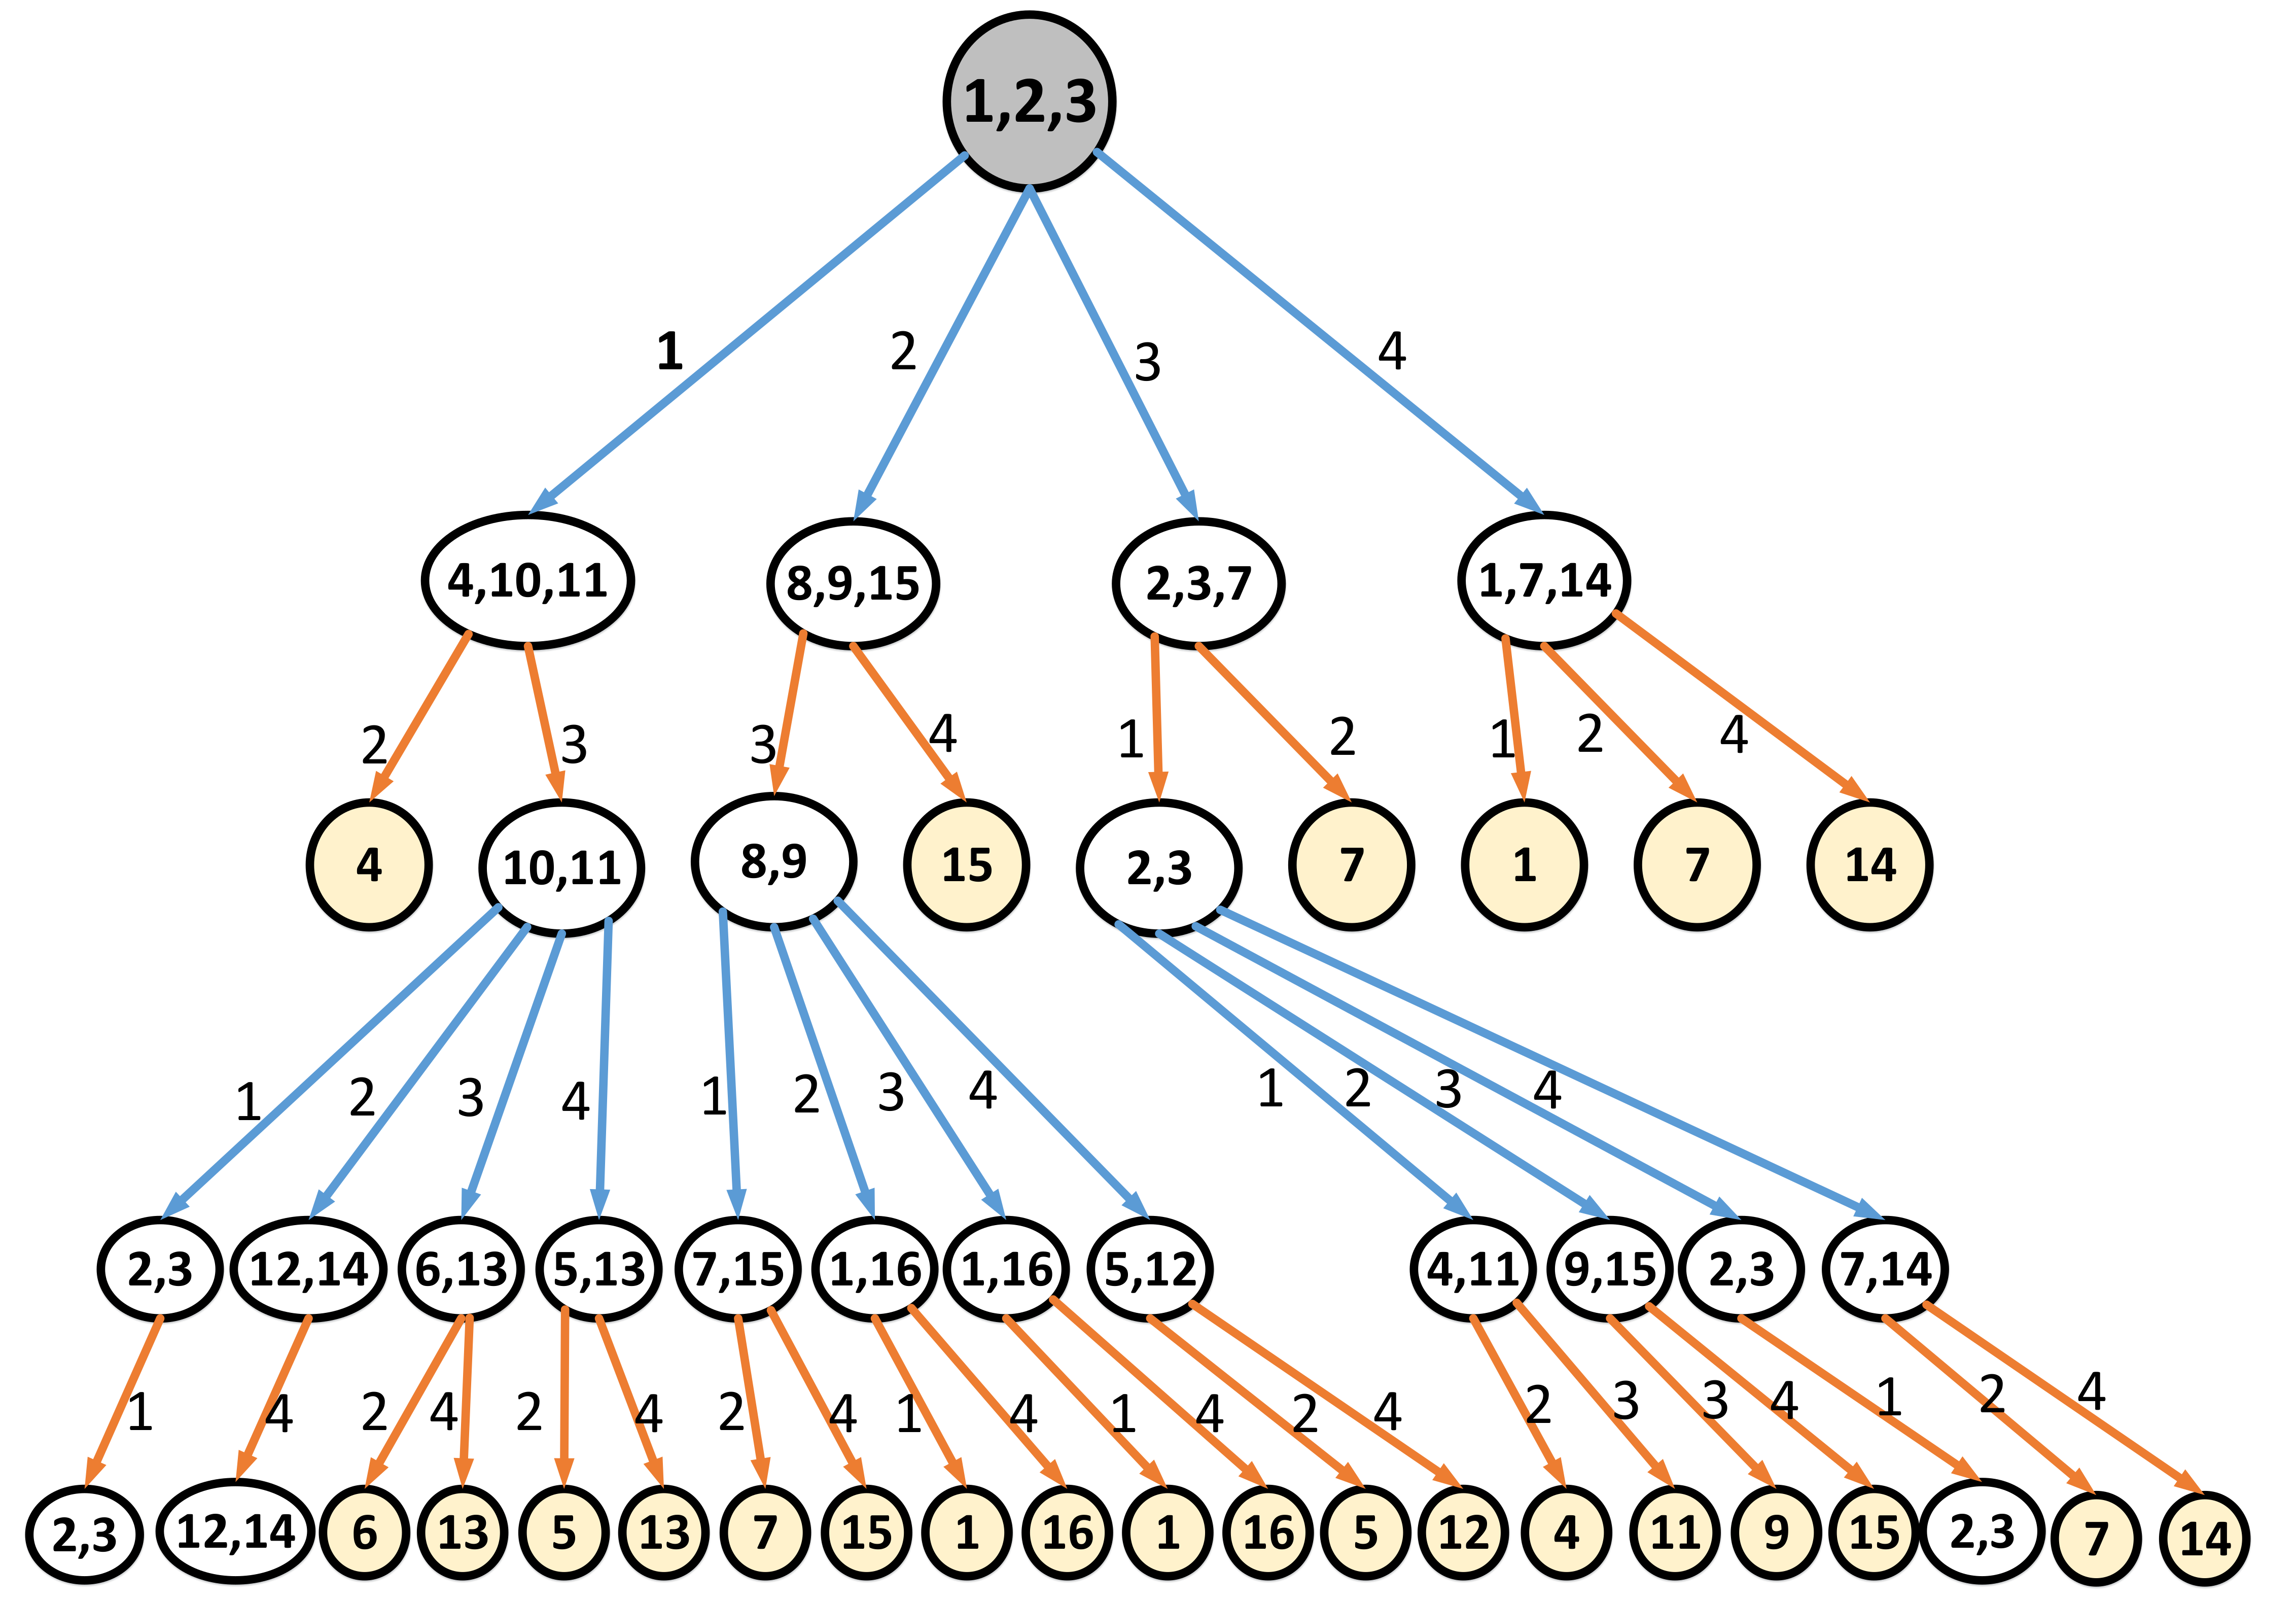
\includegraphics[scale=0.252]{figures/Fig3.png}}
	}}
      
      \caption{Branch of the super tree which represents $\{\delta_{16}^0,\delta_{16}^1,\delta_{16}^2\}$. The blue edges and orange edges show the observing output processes and deciding input processes, respectively. The yellow nodes are leaf nodes.}
      \label{fig:3}
   \end{figure}

As mentioned in the {\em Section \ref{sec:online}}, for a \BCN, we can only infer that the set of possible states is $\Delta_N$ at the beginning, thus the root node of super tree is $\Delta_N$. We can determine $\mathsf{s}(t)$ when $|\mathsf{S}(t)|=1$, thus, the leaf nodes of supertree are the nodes with cadinal number $1$. In the process of determining the $\mathsf{s}(0)$ of a \BCN, at every time step we observe the $\mathsf{o}(t)$ of the \BCN\ to derive the $\mathsf{S}(t)$ at first. After that, we decide the input $\mathsf{i}(t)$ and then preliminarily derive the new possible states set of the \BCN. Therefore we use $\Ded\left(\mathsf{S}^i,\varepsilon, \mathsf{o}^j\right)$ to find child nodes for every $\mathsf{S}^i$ in $2k+1$ layer, and using $\Ded\left(\mathsf{S}^i,\mathsf{i}^p,\varepsilon\right)$ to find child nodes for every $\mathsf{S}^i$ in $2k+2$ layer. The formula 
\[|\Ded\left(\mathsf{S}^i,\varepsilon, \mathsf{o}^j\right)|>0\]
 ensures the node $\Ded\left(\mathsf{S}^i,\varepsilon, \mathsf{o}^j\right)$ is not empty. The formula 
 \[|\Ded\left(\mathsf{S}^i,\mathsf{i}^p,\varepsilon\right)|=|\mathsf{S}^i|\] 
 guarantee we can determine the state of \BCN\ in the end. Therefore, the process of determining the initial state of a \BCN\ are depicted by the supertree, and then we can use the supertree to determine the online observability for a \BCN.

Based on the supertree, we propose the supertree-based algorithm {\bf Algorithm~\ref{alg:3}} to determine the online observability for \BCNs. In the {\bf Algorithm~\ref{alg:3}},
\begin{itemize}
\item firstly, we build the tree by breadth first. The $NodeArray$ and $NewArray$ represent the non-leaf nodes in layer $2k+1$ and $2k+2$ respectively. And we use the $TemArray$ to temporarily store the child nodes of each node of $NodesArray$ or $NewArray$ except leaf node.
\item Secondly, we check the online observability of the \BCN\ by the definition of online observability and the supertree after $2k+2$ layer of the supertree was built for every $k\ge0$. If the \BCN\ is online observable, then we stop building the supertree and delete the uncertain branches. 
\item Finally, we return the $\Delta_N$ which is the root node of the supertree, such that we can determine the initial state of the \BCN\ by the supertree.
 \end{itemize}

\begin{algorithm}[h]
\caption{Supertree-based algorithm}
\begin{algorithmic}[1]
\REQUIRE 
The updating rules of the \BCN
\ENSURE  
The super tree of \BCN
\STATE Boolean value$Ob=$ false 
\STATE integer $i$ \
\STATE integer $j$ \
\STATE integer $k$ \
\STATE nodes $NodeArray[\ ]$ 
\STATE  nodes $NewArray[\ ]$ 
\STATE  nodes $TemArray[\ ]$ 
\STATE $NodeArray[0]$ =$\Delta_N$\
\WHILE {($Ob==$ false)}
\STATE  $j=0$ \
\FOR{($i=0$; $i<arraysize(NodeArray)$; $i++$)}
\STATE  $TemArray= $ Child nodes of $NodeArray[i]$ 
\FOR{($k=0$; $k<arraysize(TemArray)$; $k++$)}
\STATE$NewArray[j+k]=TemArray[k]$
\ENDFOR
\STATE$j=j+k$
\ENDFOR
\STATE Check this \BCN\ by the super tree
\IF{(\BCN\ is online observable)}
\STATE $Ob=$ true
\ELSE
\STATE  $i=0$ \
\FOR{($j=0$; $j<arraysize(NewArray)$; $j++$)}
\IF{(NewArray[j] is not leaf node)}
\STATE  $TemArray= $ Child nodes of $NewArray[j]$ 
\FOR{($k=0$; $k<arraysize(TemArray)$; $k++$)}
\STATE$NewArray[i+k]=TemArray[k]$
\ENDFOR
\STATE$i=i+k$
\ENDIF
\ENDFOR
\ENDIF
\ENDWHILE
\STATE Delete uncertain branches

\STATE return $\Delta_N$\
\end{algorithmic}
 \label{alg:3}
\end{algorithm}

In order to better illustrate how to use the super tree to determine the online observability, we give the following example.
  
\begin{example}
For the \BCN\ mentioned in {\em Example \ref{exa:2}}. We need to determine for every \[\mathsf{o}^{j}(0)\in \Delta_Q\] such that \[|\Ded\left(\Delta_N,\varepsilon, \mathsf{o}^{j}(0)\right)|> 0,\] whether there exists a $k^{i}\ge0$ such that $\Ded\left(\Delta_N,\varepsilon,\mathsf{o}^{j}(0)\right)$ is $k^{i}$-step determinable.

Therefore, firstly we build child nodes for $\Delta_N$ by the $\Ded\left(\mathsf{S}^i,\varepsilon, \mathsf{o}^j\right)$ for every $\mathsf{o}^{j}(0)\in \Delta_Q$. For instance, \[\Ded\left(\Delta_N,\varepsilon,\delta_{4}^0\right)=\{\delta_{16}^0,\delta_{16}^1,\delta_{16}^2\},\] and at the beginning, we can not determine for $\{\delta_{16}^0,\delta_{16}^1,\delta_{16}^2\}$ whether there exists a $k^{0}\ge0$ such that $\{\delta_{16}^0,\delta_{16}^1,\delta_{16}^2\}$ is $k^{0}$-step determinable. Thus we can not determine the online observability of this \BCN\ by the supertree now. Therefore we build $2$ more layers as shown in the Fig.~\ref{fig:3}. After that, as we check the second and third layer of this branch, we have the nodes $\{\delta_{16}^0\}$, $\{\delta_{16}^6\}$ and $\{\delta_{16}^{13}\}$ are $0$-step determinable, and then we have the node $\{\delta_{16}^0,\delta_{16}^1,\delta_{16}^2\}$ is $1$-step determinable. Using the same way to check other nodes untill we can determine the online observability for this \BCN. Finally, we delete uncertain branches except the branches which can help us to determine online observability e.g. the first branch ($\{\delta_{16}^{3},\delta_{16}^{9},\delta_{16}^{10}\}$) in the Fig.~\ref{fig:3}. 
\label{exa:11}
\end{example}   

However, if we want use the supertree-based algorithm to find all paths to determine the initial state of a \BCN\ we need to build all leaf nodes of its supertree. It would take many additional time and space overhead. Because 
 there are many nodes take identical set of states in the supertree, such that we need to check them many times to determine the online observability of a \BCN. 
 
 What is more, the nodes contain identical set of states in a path may prevent us from building all leaf nodes of the supertree. For instance, there are three nodes take $\{\delta_{16}^1,\delta_{16}^2\}$ in a path as shown in Fig.~\ref{fig:3}, in this case, $\{\delta_{16}^1,\delta_{16}^2\}$ has infinite number of successor nodes. Therefore, we can not build all successor nodes for it, and then we can not build supertree completely.

 
With the shortcomings of the supertree, we propose the algorithm based on directed graph to help us find all paths to determine the initial state of a \BCN.
\subsection{Algorithm based on directed graph}
The directed graph is used to depict the process of determining the initial state $\mathsf{s}(0)$ of a \BCN\ too. 
For convenience, we also use the set of states ($\mathsf{S}^i$) inside a node to represent this node, and the input ($\mathsf{i}^p$) on an edge to represent the edge.  
Therefore, we have the definition of directed graph for \BCNs.
\begin{definition}[Directed Graph]
For the directed graph of a \BCN.   
\begin{itemize}
\item The nodes of the directed graph are the nodes which satisfy that.
\begin{itemize}
\item  The node $\mathsf{S}^i$ that there exists a $k^{i}\ge0$ such that $\mathsf{S}^i$ is $k^{i}$-step determinable.
\item When $|\mathsf{S}^i|>1$, for every distinct two $\mathsf{s}^x, \mathsf{s}^y \in \mathsf{S}^i$, $h(\mathsf{s}^x)=h(\mathsf{s}^y$). 
 \end{itemize}

\item The edges of directed graph satisfy that.
\begin{itemize}
 \item If $|\mathsf{S}^i|=1$, then there are not edge from $\mathsf{S}^i$ to other nodes.
 \item  If $|\mathsf{S}^i|>1$, then if for a $\mathsf{i}^p$ we have \[|\Ded\left(\mathsf{S}^i,\mathsf{i}^p,\varepsilon\right)|=|\mathsf{S}^i|,\] and every $\Ded\left(\mathsf{S}^i,\mathsf{i}^{p},\mathsf{o}^{j}\right)\ne\emptyset$ is a node of the graph. Then there exists an edge $\mathsf{i}^p$ from $\mathsf{S}^i$ to every $\Ded\left(\mathsf{S}^i,\mathsf{i}^{p},\mathsf{o}^{j}\right)$.

 \end{itemize}
 \end{itemize}
\end{definition}

Comparing with supertree, in the directed graph, the states in the same node $\mathsf{S}^i$ with idential corresponding output. Thus, we do not need represent the process of observing output by an edge. And every node $\mathsf{S}^i$ appears only once, such that the directed graph has finite number of nodes. And then we can build the directed graph completely by $\Ded\left(\mathsf{S}^i,\mathsf{i}^{p},\mathsf{o}^{j}\right)$. Therefore, we use the directed graph to help us find all paths to determine the initial state of a \BCN.

From the {\em Lemma \ref{lemm:2}} in the {\em Section \ref{sec:online}}, we have that if for the set of states $\mathsf{S}^x$ there does not exist any $k^{1}\ge 0$ such that $\mathsf{S}^{x}$ is $k^{1}$-step determinable, and $\mathsf{S}^{x}\subseteq \mathsf{S}^{y}$. Then there does not exist a $k^{2}\ge 0$ that make $\mathsf{S}^{y}$ $k^{j}$-step determinable. Therefore, in the process of building the directed graph for a \BCN\ we build the nodes with fewer states at first, and then build the nodes with more states.
\begin{itemize}
\item  Because, once we can find node $\mathsf{S}^i$, such that there does not exist any $k^{i}\ge0$ makes $\mathsf{S}^{i}$ $k^{i}$-step determinable. And we know that there exists $\mathsf{o}^{j}\in \Delta_Q$ such that $\mathsf{S}^{i}\subseteq \Ded\left(\Delta_N,\varepsilon, \mathsf{o}^{j}\right)$. Thus, we have for $\Ded\left(\Delta_N,\varepsilon, \mathsf{o}^{j}\right)$, there does not exist any $k^{j}\ge 0$ that makes  $\Ded\left(\Delta_N,\varepsilon, \mathsf{o}^{j}\right)$ $k^{j}$-step determinable either, and then the \BCN\ is not online observable.
\item And as we determine the $k$-step determinability of every $\Ded(\mathsf{S},\mathsf{i}^{i},\mathsf{o}^{j})$, we can determine the $k$-step determinability of $\mathsf{S}$ easily.
\item  Finally, as the $k$-step determinability of the subsets of $\mathsf{S}$ has been checked, it is convenient for us to find the $\mathsf{i}^{i}$ which makes $\mathsf{S}$ $k$-step determinable by the subsets of $\mathsf{S}$.
 \end{itemize}
 
With the definition of directed graph and the way to construct the derected graph. We propose the algorithm based on directed graph {\bf Algorithm~\ref{alg:1}}, and the {\bf Algorithm~\ref{alg:2}} to build nodes which is used in the {\bf Algorithm~\ref{alg:1}}.

\begin{itemize}
\item  Firstly, for every $k>0$ we try to build nodes with $k$ states, and the states with identical corresponding output. And we use the $NodeArray$ to represent them.
\item Secondly, if the nodes can  be built, when $k>1$, we check the determinability of every node and build edges for them. And, if we can not build any edge for one of them, we have the \BCN\ is not online observable.
\item Fianlly, if we can not build any node with $k$ states, then we have the determinability of all of the set of states have been checked. Thus the \BCN\ is online observable, and {\bf Algorithm~\ref{alg:1}} returns the $\Delta_N$.
 \end{itemize}

\begin{algorithm}[h]
\caption{Algorithm based on directed graph}
\begin{algorithmic}[1]
\REQUIRE 
The updating rules of \BCN
\ENSURE  
The directed graph of \BCN
\STATE Bool ean value$Ob=$ true 
\STATE integer $i$ \
\STATE integer $j$ \
\STATE integer$k=1$ 
\STATE nodes $NodeArray[\ ]$
\STATE inputs $InputArray[\ ]$
\STATE {\sf buildnode}(k)
\STATE $k= k+1$
\STATE $NodeArray=${\sf buildnode}(k)
\WHILE {($NodeArray!=$Null)}
\FOR{($i=0$; $i<arraysize(NodeArray)$; $i++$)}
\IF{($k==2$)}
\STATE $InputArray$ = $\Delta_M$ 
\ELSE

\STATE Find $InputArray$ by other nodes

\ENDIF
\FOR{($j=0$; $j<arraysize(InputArray)$; $j++$)}
\STATE Check $NodeArray[i]$ by $InputArray[j]$ 
\STATE Build edges for $NodeArray[i]$ 
\ENDFOR
\IF {($NodeArray[i]$ has not any edge)}
\STATE  $Ob=$ false 
\STATE return Null
\ENDIF
\ENDFOR
\STATE $k= k+1$
\STATE $NodesArray=${\sf buildnode}(k)
\ENDWHILE
\STATE return $\Delta_N$\
\end{algorithmic}
 \label{alg:1}
\end{algorithm}
\begin{algorithm}[h!]
\caption{{\sf buildnode}(int k)}
\begin{algorithmic}[1]
\REQUIRE 
The number of states $k$
\ENSURE  
The nodes with $k$ states which with the same corresponding outputs 
\STATE  Build all nodes with $p$ states 

\IF{(Failed to build)} 
\STATE  return Null
\ELSE 
\STATE  Classify these nodes
\STATE Sort the states in these nodes
\STATE Sort these nodes
\STATE return nodes
\ENDIF 
\end{algorithmic}
 \label{alg:2}
\end{algorithm}

There are some details in {\em Algorithm.\ref{alg:1}} and {\em Algorithm.\ref{alg:2}} are as follows:
\begin{itemize}
\item Build all nodes with $k$ states:
\begin{itemize}
\item Firstly, we classify all states by their corresponding outputs. Then we can get the set which contains all states with identical corresponding output i.e. $\Ded\left(\Delta_N,\varepsilon,\mathsf{o}^{j}\right)$.
\item Secondly, we compare $k$ with each $|\Ded\left(\Delta_N,\varepsilon,\mathsf{o}^{j}\right)|$. If $k>|\Ded\left(\Delta_N,\varepsilon,\mathsf{o}^{j}\right)|$, then we could not get any set with $k$ states from $\Ded\left(\Delta_N,\varepsilon,\mathsf{o}^{j}\right)$. Else we can get $\frac{(|\Ded\left(\Delta_N,\varepsilon,o_j\right)|)!}{k!\times (|\Ded\left(\Delta_N,\varepsilon,o_j\right)|-k)!}$ sets of states, where $k!$ is the factorial of $k$.
\item Finally, we use all of the sets of states found in second step to build nodes. 
\end{itemize} 
 \item Sort the states in these nodes and sort these nodes: We sort the states inside the nodes at first, and then sort the nodes by the states of them. For example, in Fig.~\ref{fig:4} the nodes $\{\delta_{16}^0,\delta_{16}^1\}$, $\{\delta_{16}^0,\delta_{16}^2\}$ and $\{\delta_{16}^1,\delta_{16}^2\}$ are well shorted. 
  \item 
   For the node $NodeArray[i]$ contains $k$ sorted states, we can use the node with the first $(k-1)$ states of $\mathsf{S}^i$ and the node with the last $(k-1)$ states of $\mathsf{S}^i$ in the directed graph to find $InputArray$ for $NodeArray[i]$. For example, we can search the edges which from $\{\delta_{16}^3,\delta_{16}^4,\delta_{16}^5\}$ and $\{\delta_{16}^4,\delta_{16}^5,\delta_{16}^6\}$ at first. And then, take the intersection of this two sets of edges to be $InputArray$ of $\{\delta_{16}^3,\delta_{16}^4,\delta_{16}^5,\delta_{16}^6\}$. 
  \item Check $NodeArray[i]$ by $InputArray[j]$:
     
\begin{itemize}
\item If for the $InputArray[j]$ and $NodeArray[i]$ we have that $|\Ded\left(NodeArray[i],InputArray[j],\varepsilon\right)|<|NodeArray[i]|$, then we can make sure the $InputArray[j]$ is a wrong input.
\item Else if every \[\Ded\left(NodeArray[i],InputArray[j],\mathsf{o}^{p}\right)\ne\emptyset\] already exists in the directed graph, then if $NodeArray[i]$ does not exist in the graph yet, we contruct it, and then connect it to every $\Ded\left(NodeArray[i],InputArray[j],\mathsf{o}^{p}\right)$ with the edge $InputArray[j]$.
\item Else if there exist a node \[\Ded\left(NodeArray[i],InputArray[j],\mathsf{o}^{p}\right)\] has not been constructed yet, then we check it latter. 
\end{itemize} 
\end{itemize} 

\begin{figure}[thpb]
      \centering
      \framebox{\parbox{3in}{
		\centerline{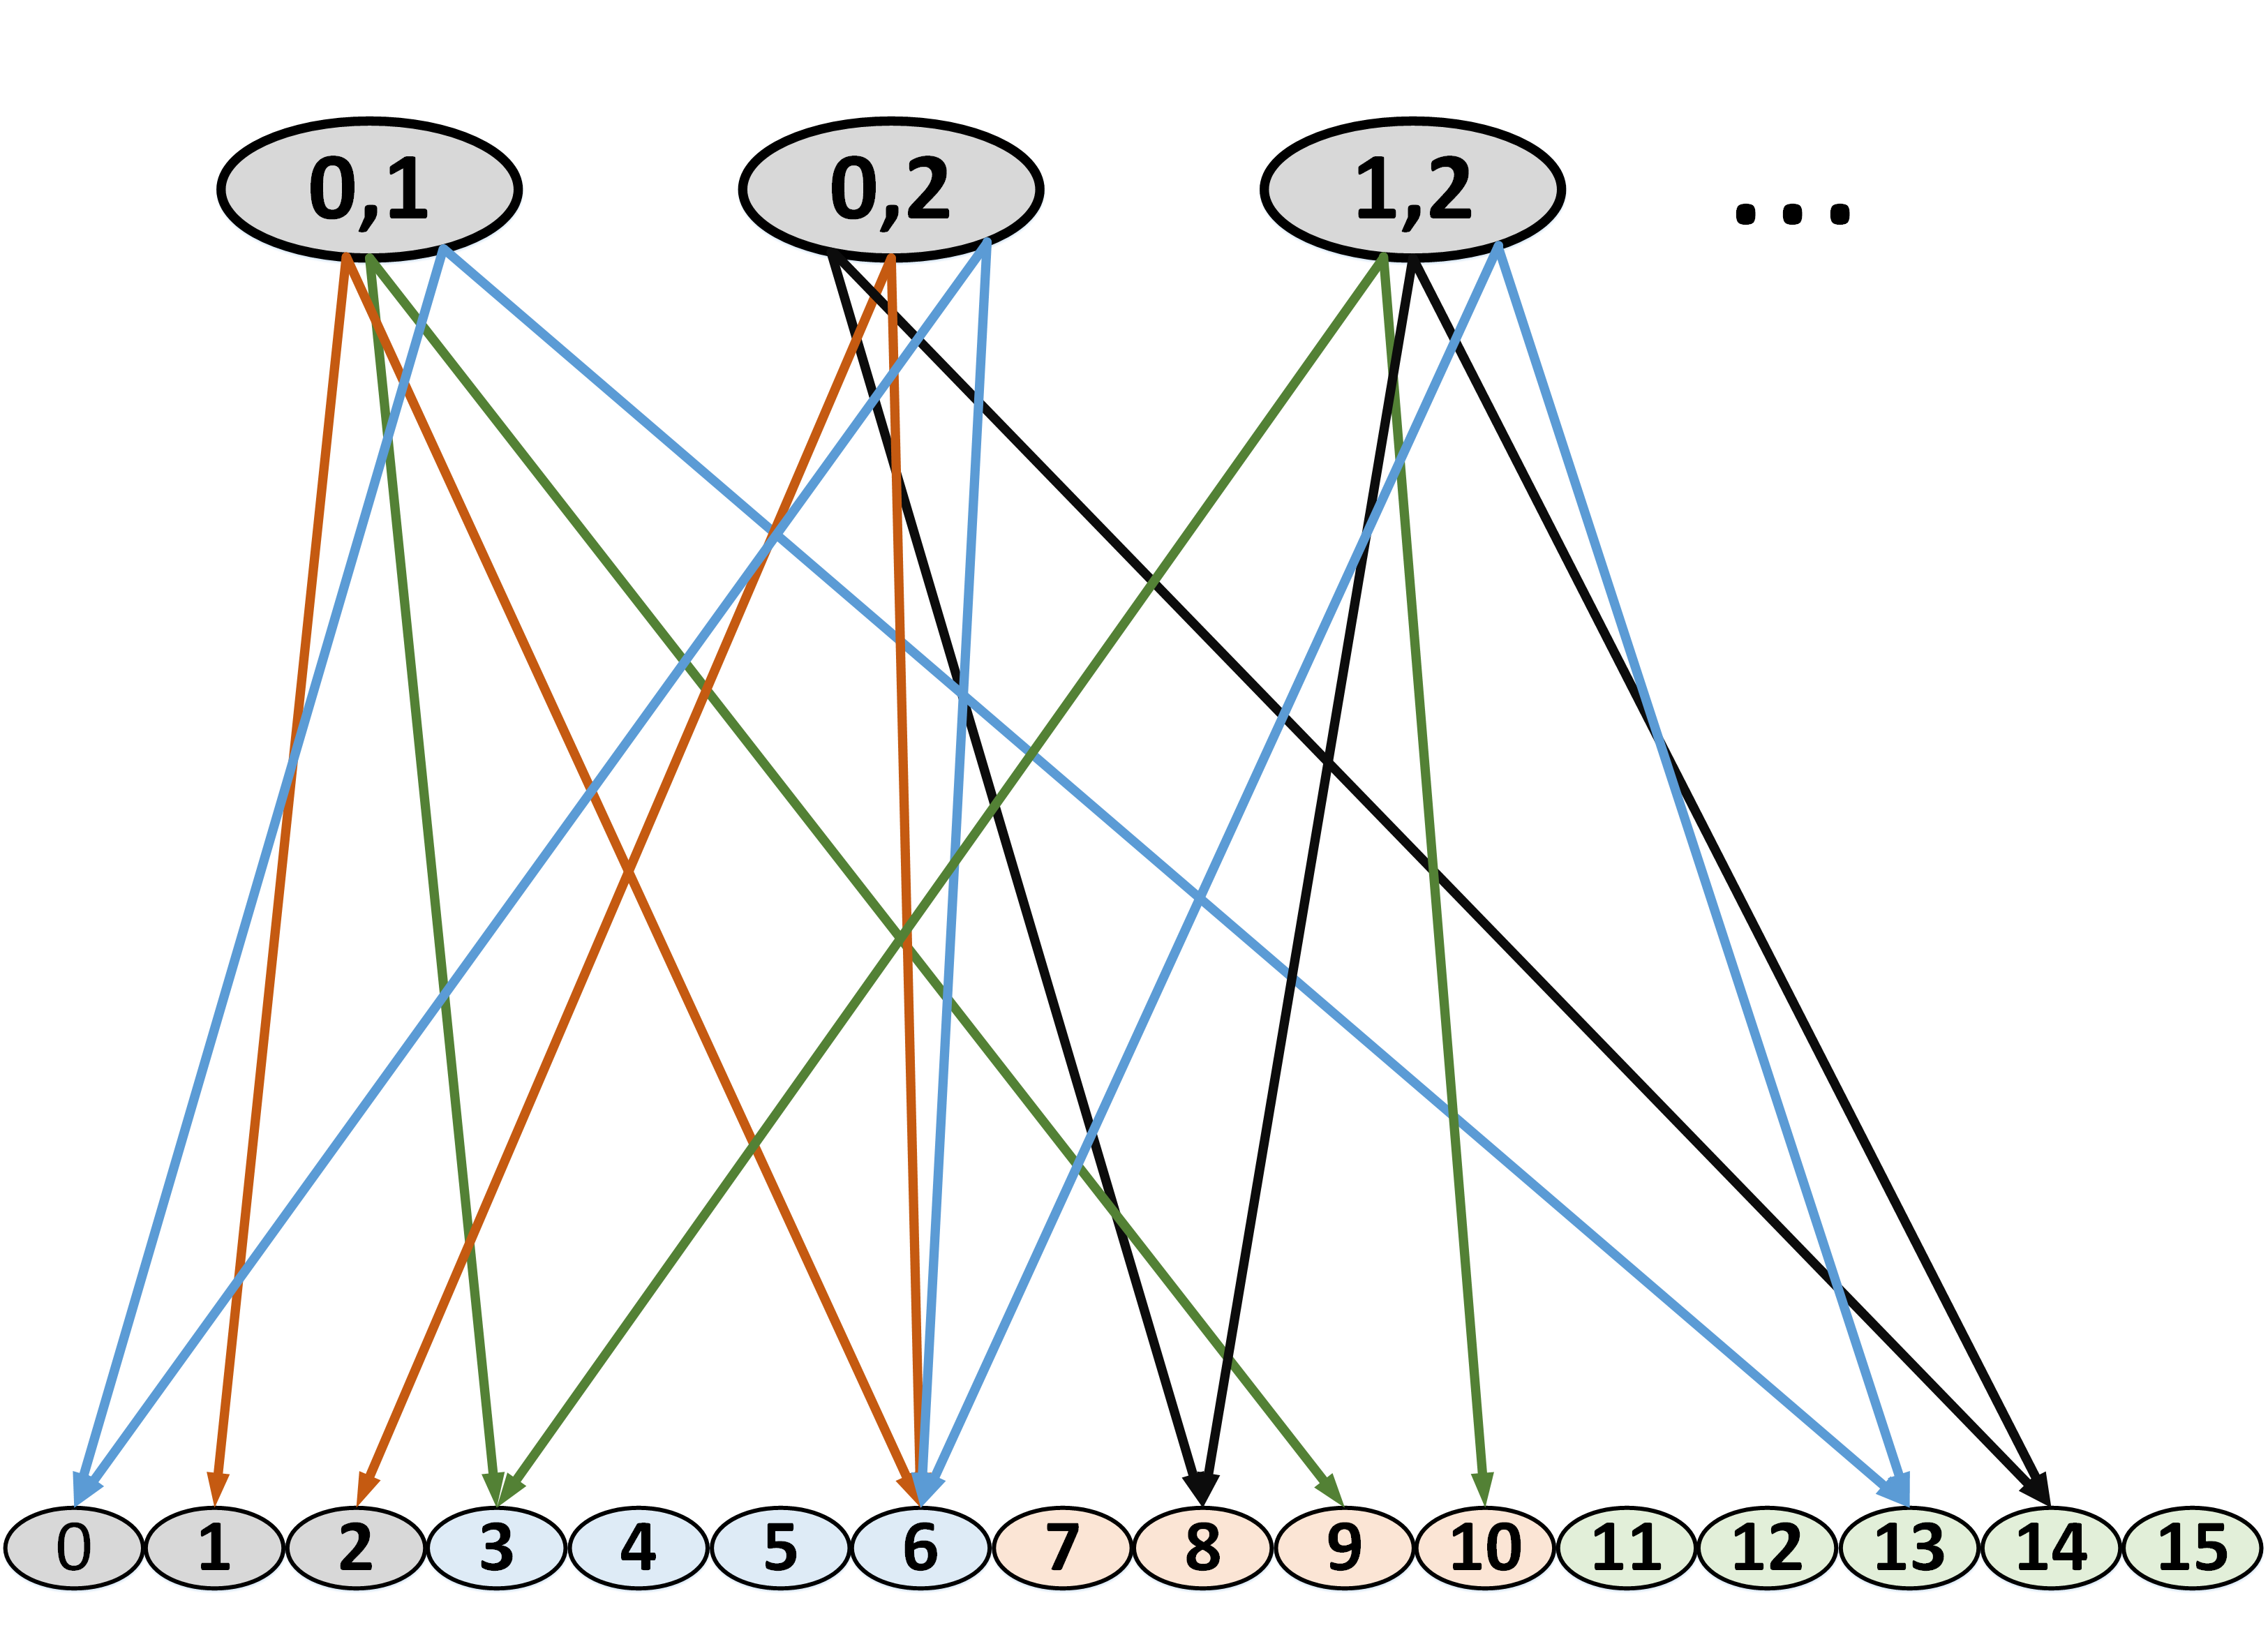
\includegraphics[scale=0.090]{figures/Fig4.png}}
	}}
      
      \caption{Part of the directed graph which represents $\{\delta_{16}^0,\delta_{16}^1\}$, $\{\delta_{16}^0,\delta_{16}^2\}$ and $\{\delta_{16}^1,\delta_{16}^2\}$. The green, black, orange, blue edges show the inputs $\delta_4^0$, $\delta_4^1$, $\delta_4^2$ and $\delta_4^3$ respectively.}
      \label{fig:4}
   \end{figure}

With the algorithm based on directed graph we can find all paths to determine the initial state of a \BCN. Thus, at time step $t$, we can use the $\mathsf{S}(t)$ and the directed graph to derive all of the input $\mathsf{i}(t)$ which can help us determine $\mathsf{s}(0)$. While, there comes a problem. Which input is the best input? To solve this problem, in the {\em Section \ref{sec:app}}, we will present how to decide the input to get better performance.
